\documentclass[a4paper, 10pt]{article}

\usepackage{graphicx}
\usepackage{hyperref}

\hypersetup{
	colorlinks=true,
	linkcolor=blue,
	filecolor=magenta,
	urlcolor=cyan,
	citecolor=green,
}

%Replace title
\title{Mimir Iteration 1 Standard Notes}
\date{\today}

\begin{document}
\maketitle

\pagebreak

\tableofcontents

\pagebreak

\section{Chassis Design}
This section covers the design of the Mimir chassis. The chassis includes mounting for all devices and motors. This is a mostly mechanical section. 

	\subsection{NO DATE: Catchup}
		\subsubsection{Summary}
		To date no notes have been taken, and much work has been done. Much in the way of previous design review has been completed. Some resource books have been read and the major takeaways are included below. Combined with previous design review and reading a list of considerations is created.
		
		Early design decisions were explored, based on previous designs, available resources, and some information learned out of books. Since motors are expensive and we're not looking to blow any more of our budget, they dictate the design; we will ideally use the fastest, 612 RPM motors, though backups/alternatives are the 118RPM ones. Details of the power systems were provided below with rationalization. 
		
		Early thoughts on the network stack were discussed lightly. A dedicated network section was created.
		
		\subsubsection{Roadblock: Brushing up with good resources}		
		The lack of documentation from previous year's teams, and the dearth of UWB mechanical design education makes designing a rover hard or almost impossible. I scraped through websites, forums, and catalogs of books to try and find the best I can on rover design and drive train design. The two most important books I've read so far in order were \textit{Making Things Move} by Dustyn Roberts and \textit{Building Robot Drive Trains} by Dennis Clark, both included in the references section for this document. The former can be found on LibGen, the latter is almost impossible to find online or Amazon, and I had to get my copy from Ebay. There's also another book by Dennis Clark about building robot bases which I didn't find useful, but which might be good for absolute beginners.
		
		\textit{Making Things Move} is an absolute beginner book and provides great resources on component outlets, basic concepts, and some useful design tips for selecting/mounting motors. 
		
		\textit{Building Robot Drive Trains} is incredibly in depth while being beginner friendly. I went through chapters 1-3, 6, and 10, as I needed; but, electrical and control engineers should go through chapters 7-9. If you ever need pointers on stepper or servo motor selection/control do chapters 4-5. 
		
		\subsubsection{Roadblock: Early decisions, priority considerations, and future work}
		Some early design decisions are based on available materials and what's worked. The list of electronic components is:
		\begin{itemize}
			\item Nvidia Jetson Nano
			\item The Power Distribution System (PDS)
			\item Two buck modules
			\item Two batteries
			\item The Arduino, motor controllers, and other headers mounted to the PDS
			\item The Stewart platform (SP)
			\item The SP's power/signal distribution board and Arduino controller
			\item An unknown subset of wireless devices, see below section... 
		\end{itemize}
		We're ideally going to be going with our fastest, 612RPM motors, though the next backup and alternative is 118RPM. Early designs will obviously be slower than desired, but future updates will use 3D printed gears to gear up the speed. Batteries will power the system through a dangling wire, through the buck modules - mounted somewhere on the frame - then into the PSU. The PSU needs a 2.5 inch clearance, after considering thickness and the tallest component (the motor controllers). 
		
		The first iteration is largely going to emphasize re-purposing the existing system to include more components with better mounting. Some additional thought is going to be given to improving the treads. Unfortunately - as mentioned above in the section on design review - it appears last year's team used M3 sized through holes and fasteners for their standard, while the previous year's team used M2. This isn't a huge deal, (since M2 can be used on an M3 frame), but will make the design a bit trickier. A future section will be dedicated to a design review.
		
		Since the motor dictates the design we have to get its data sheet, (see references below). Note to self that the data sheet folder in the drive needs a severe organization. All literature advises over-sizing motors and running them at 10-20\% their stall torque in continuous run, split the difference and we should be working at 15\%; further analysis will get a more precise value. This makes sense as maximum efficiency occurs roughly at 15\% stall torque; we want to minimize battery drain. Doing this will set both the speed and torque output, the latter which will determine the weight of the rover. We don't expect the first iteration to drive up stairs, but when future iterations do, the incline increases net torque experienced; still we hope this won't creep up past 20\%. Obvious future changes could be to accept normal operating torque of 10\% of stall after reducing weight. The calculations for experienced forces driving up stairs in extreme conditions and on flat terrain still need to be completed at this stage. This does bring up a tangent point: we must consider implementing a geared transmission with a shifter so we can travel up stairs more efficiently. 
		
		The operation of the motor is also intimately related to travel speed and power consumption. We must determine early if the planetary gear motors provided by RobotZone have already considered losses to inefficiencies of gears, and how that will affect power consumption, but not sure this is possible. The rover travel speed is based on the diameter and angular speed of the tank drive sprocket. The angular speed of the tank drive sprocket is the motor's angular speed, which is not actually 612RPM, despite being named so. Remind yourself that 612RPM is the no-load speed (this particular motor has 10\% uncertainty by the way) and this decreases linearly with increasing torque. Operating at 15\% torque we should actually expect to see 520RPM (85\% speed). I will soon create accurate (enough) motor curves for reference, and calculate exact parameters on torque experienced and maximum weight allowed. Useful calculations can be found in Dennis Clark's \textit{Building Robot Drive Trains}. 
		
		For this first iteration we want to use the existing base, but build the ideal component mountings. The priority future changes are improved tank treads, and weight distribution. The current tank treads are made of a smooth material ideal for traveling indoors on flat ground; these treads should be swapped out for our rubber-clad treads (in the locker). The rubber will improve grip and permit us to travel up stairs. What's more is the need for a 'complex' tank tread design, we're limited with the existing drive and idler sprocket setup. With only idler/drive sprockets the bottom tread doesn't make meaningful contact with the ground. By adding bogies - small, often spring-engaged wheels - to apply force to the bottom face of the treads, we can increase the experienced force of friction, improving traction. Furthermore, the bogies will create tighter, more rigid 'kinks' in the chain of treads, giving better 'grab' on the stairs. At this point I haven't determined the existing weight of the rover, nor compared it against allowable weight. If I find it's already optimized for the efficient torque, future iterations will need to cut down on drive base weight. If we find it's below optimal efficiency, the component mounting should 'brush up' against max allowable weight (so we don't have to pay much mind in the future). If it's far above optimal efficiency, the entire system should be completely redesigned at a later point, little mind needs to be paid to weight of the component mounting scheme as it wouldn't matter now. The weight distribution also needs to consider 3D center of gravity (ideally low and center), and the relation of the electronics stack to the treads. 
		
		\subsubsection{Roadblock: Network stack confusion}
		Right now I'm not entirely sure what the network stack was supposed to be. Most of the information is entirely theoretical or poorly physically implemented. I have a slough of mango, WiFi mini routers, a Linksys VPN router, another Linksys wireless, broadband router, and a NETGEAR gigabit ethernet switch. Currently I'm taking Networking as part of my computer science minor, so I hope in the next few weeks I'll be equipped with the knowledge to make more informed selections. Any further discussion will be held in it's own section.	
		
		
	\subsection{5/7/23}
		\subsubsection{Summary}
		Motor curves were generated for the candidate motors, and appreciable discussion was had. The short of it: previous teams were incredibly lazy in motor selection and we're probably operating at incredibly inefficiency. We need to up the torque on our motors, or reduce our weight, or both; the rover will likely see a drop in speed, but it won't be significant. Some additional force analysis and quick estimates of weights were provided. 		
		
		\subsubsection{Roadblock: Generating non-existent motor curves}
		Motor curves are simple plots of torque vs current, power, speed, and efficiency. Speed is inversely proportional to torque, with the maximum value being the no-load speed (written on the motor) occurring at 0 torque, and the minimum value being 0 at stall torque. We have two potential motors for use, so I'll generate the curves for both: 612RPM and 118RPM motors.
		
		The current has no-load and stall torque values; for our particular 612RPM (or 64.08 rads/sec) these are 0.5A (no-load) and 20A (stall). Mechanical power can be found as the product of torque (Nm) and angular velocity (rads/sec); this is different than electrical power, which is the product of applied voltage and drawn current. Efficiency is the ratio of mechanical power (output) to electrical power (input). Stall torque is 16kgF-cm, or about 1.57Nm.
		
		With the above parameters I used Desmos to plot the motor curve of our selected motor. Torque units are in Newton meters, rotational velocity (red line) units are in rads/sec, mechanical output power (green) are in Watts, current (blue) is in amps. The \textbf{efficiency (black) has been multiplied by a factor of 50} for easy visualization; correcting and we see a maximum of 31.25\% efficiency at $ 0.21/1.57 => 13.37\% $ of the stall torque.
		
		\begin{figure} [!h]
			\centering
			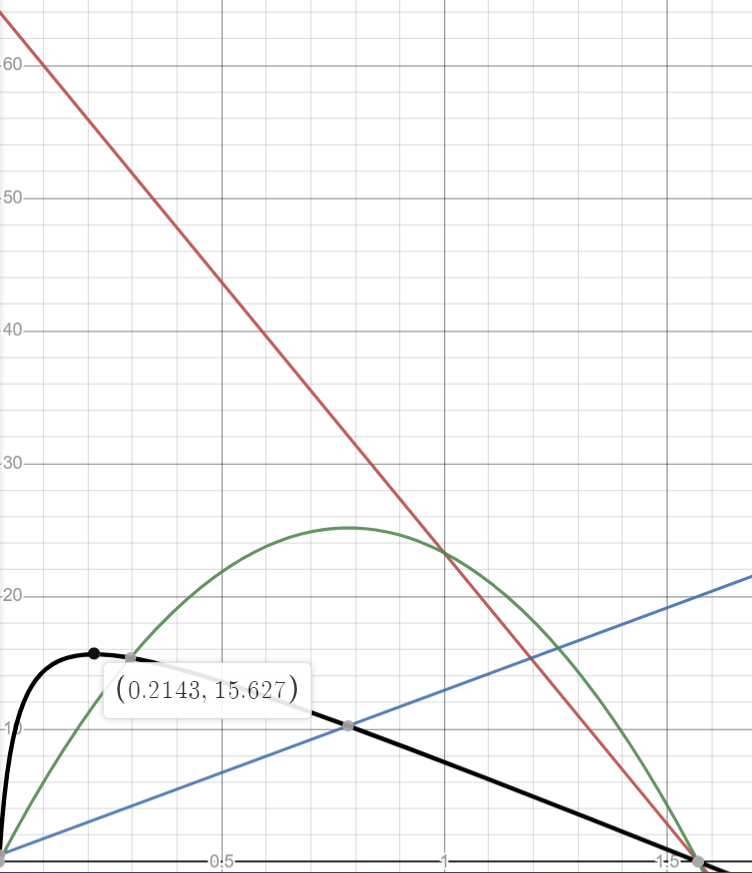
\includegraphics[scale=0.5]{motor_curves_612}
			\caption{Motor curves with efficiency multiplied by a factor of 50 for scale}
			\label{motor_curves_612}
		\end{figure}
		
		For our 118RPM (or 12.35 rads/sec) current values are 0.5A (no-load) and 20A (stall). Stall torque is 69kgF-cm, or about 6.76Nm. 
		
		With the above parameters I used Desmos to plot the motor curve of our selected motor. Torque units are in Newton meters, rotational velocity (red line) units are in rads/sec, mechanical output power (green) are in Watts, current (blue) is in amps. The \textbf{efficiency (black) has been multiplied by a factor of 20} for easy visualization; correcting and we see a maximum of 26.05\% efficiency at $ 0.927/6.79 = 0.1365 => 13.65\% $ of the stall torque. 
		
		\begin{figure} [!h]
			\centering
			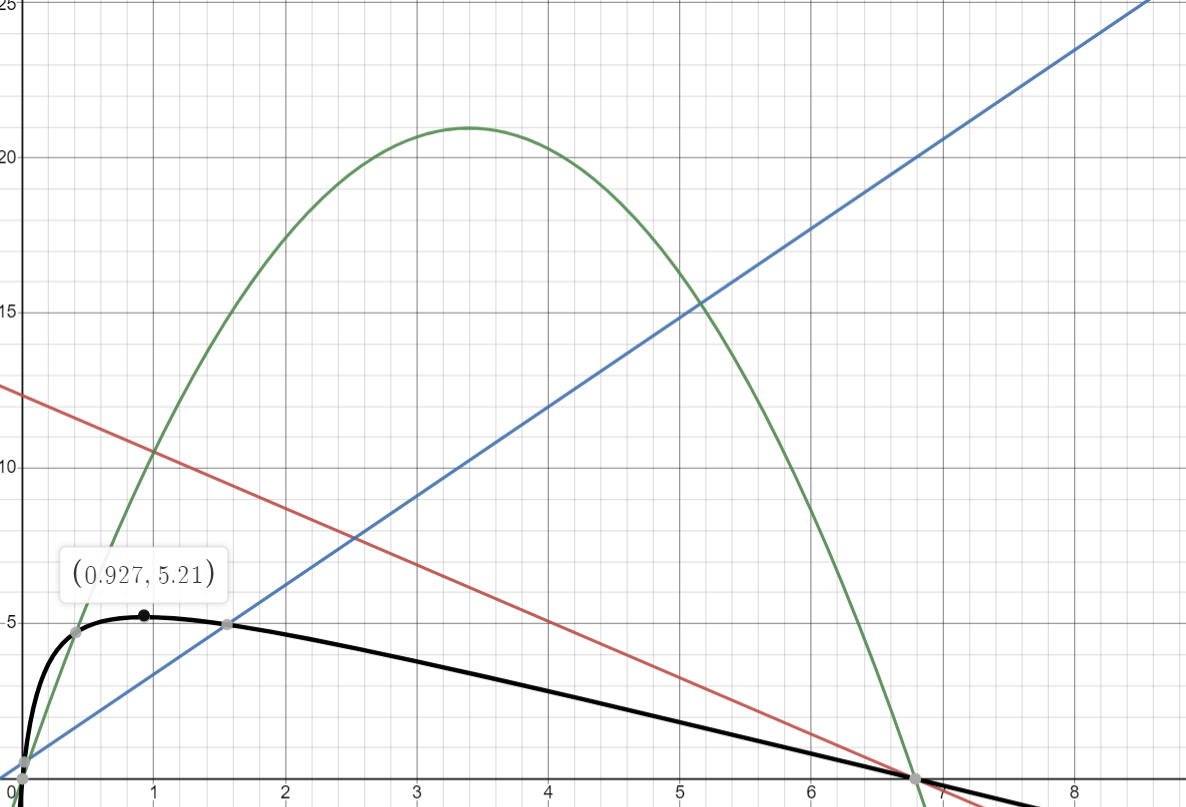
\includegraphics[scale=0.5]{motor_curves_118}
			\caption{Motor curves with efficiency multiplied by a factor of 20 for scale}
			\label{motor_curves_118}
		\end{figure}
		
		\subsubsection{Roadblock: Determining torque, maximum allowable size, and speed}
		See the motor curves above for useful context. When considering the 612RPM motors, we've determined a maximum efficiency of 31.25\% if we run the motor at 13.37\% of the stall torque, which is about 0.214Nm. 
		
		At 13.37\% of the stall torque, we'd be running 86.63\% of the no-load speed, or 526RPM, which is 55 rads/sec. The velocity of a tank tread is simply the linear velocity of it's drive sprocket. The current design, which we're building on uses 2400 Series goBUILDA tracks, and a 100mm diameter sprocket; thus linear velocity is $v = 55rad/s * 50mm$, a reasonable 2.75 meters per second, or a little over 8 feet per second. 
		
		If we assume we're going to drive this rover entirely flat at the maximum efficiency, our motor should experience 0.214Nm of torque. When moving a single 50mm radius sprocket, the force developed at the contact is 4.28 Newtons. From here things are a bit confusing, as from first glance the rover appears to have two of these motors, but the document (which is admittedly outdated) shows 4. If we have 2 our total force propelling the rover is 8.56 Newtons, 4 and it's 17.l2 Newtons. Move past the motors for a moment and determine what our rover must overcome to move. Consulting some literature, a liberal frictional coefficient for tread based vehicles should be 0.5 the weight; 0.7 will be our conservative. I'm also going to do the calculations for the rubber tank treads we might use in the future at 0.9 (around the value of rubber on dry concrete). The tank treads never roll, so static friction is a constant. The force to overcome is thus 
		$$F_{app} = \mu mg$$
		We can assume that the motor will match this force, and solve for the only unknown (our mass). If we assume two motors outputting 8.56 Newtons: at the liberal friction coefficient estimate our ideal weight should be 1.75kg (3.8lbs), while for the conservative it should be 1.25kg (2.75lbs), and the future rubber treads about 0.97kg (2.13lbs). Obviously this is a massive weight reduction from the current 25 lbs rover, which would cause the motors to deliver 88\% its stall torque, an incredible inefficiency. I really want my math to be wrong, but nothing from their MegaDoc explains the decisions they made. If we assume 4 motors and 17.12 Newtons, then the ideal weight should be liberal - 3.5kg (7.9lbs), conservative - 2.5kg (5.5lbs), and future - 1.94kg (4.26lbs); again this is a huge difference from the realistic 25 lbs rover, which would require the motors to deliver 44\% its stall torque. Remember, our goal is 13\%... Trying to read back through their document I see mention of a speed test, but they placed the data into an image that got corrupted and never submitted with the PDF. There is one mention I saw of 1.1m/s, and while I don't think it's the rover they built, it would correspond to about 70\% of stall torque, causing me to lean on the side of 2 motors. I think what happened was this last team wanted a faster rover, and mindlessly piggybacked off the year-prior team's decision to use 118RPM motors without considering the torque specifications of the rover. If that rover uses 2 motors instead of 4, it's damn near a miracle it works, and it certainly wouldn't work climbing stairs. 
		
		The guaranteed takeaways are: (1) we need to drastically reduce the weight as much as possible to reach peak efficiency, or (2) we need to swap out the motors for 118RPM motors which will result in improved efficiency, and possibility to climb stairs. Fortunately most of the logical components don't amount to collectively more than a pound, leaving between 4 and 6 pounds for the rest of the chassis, batteries, and Stewart platform. 
	
		Another future consideration is performance on stairs. The equation used above was flat only, however it would become 
		$$F_{app} = \mu mgsin\theta + mgcos\theta$$
		for traveling up an incline of $\theta$ degrees. The increase here is appreciable when you consider how steep Discovery Hall's stairs are. Even 4 612RPM motors would be pushing their luck, we'd prefer 4 118RPM motors. 
	
		\subsubsection{Roadblock: Dividing the Iteration 1 Design}
		I'd still like this first iteration to include the Stewart platform; but, time for implementation gets in the way. \textbf{Pay attention when reading these notes and consider} that I'm designing the entire iteration 1 rover with weight consideration for the Stewart platform, but not including it at the outset. Instead I'm going to design a simple mounting so the software team can begin testing. The next few days may include notes that make little mention to the Stewart platform, but the later days will. 
		
		From that point on these Roadblock sections will be visibly split between my work on the chassis and Stewart platform, and only near the end will they come together. More info on the Stewart platform will be contained in its own document.

		
	\subsection{5/8/23}
		\subsubsection{Summary}
		Completed a basic design review of some of the past projects, and discussed an improved estimate of the weight max and some other parameters.
		
		\subsubsection{Roadblock: Much needed design review}
		HackRover has existed for many years, and has seen the creation of multiple rover systems of a variety of designs. There are three distinct tracts in the history: (1) the 'HackRover Games' era, the (2) NASA rover design attempt, and (3) the current HARC event and disaster relief rover theme.
		
		Looking back at the designs of the HackRover games we see bulky, extremely redundant, sprawling systems with massive weight, (upwards of 40lbs). Attempt at stair climbing extensions never worked and just added weight. The drive train consisted of motors mounted at their heads only (no supportive shims anywhere else), and long, skinny shafts with set screw collars. These shafts bent and marred. Almost all fasteners were black oxide, button head cap, M2 screws. The motors were usually well sized, experiencing about 30-40\% the stall torque (certainly not the ideal 13\% spoken of before), but exhibiting 20-25\% efficiency on motors whose max efficiency was only 27\% anyways. Treads were high friction coefficient (0.9 and up) rubber, and pretty narrow. There was also a small sub team that attempted to design a rover with mecanum wheels, which failed; they blew their entire budget on 20+ mecanum wheels we're yet to use. The mechanical designs were all right, and practice good enough. The greatest boon of this phase was the amount of materials we accrued. The major takeaways were to: (1) cut weight where it's not absolutely necessary, (2) cut way by performing stress analysis with simulation software, (3) use shorter shafts, (4) improve motor mounting, (5) don't use set screw collars, but opt for clamp collars instead, and (6) improve shaft component mounting techniques to not cause damage.
		
		Looking back at the designs of the NASA rover we see a sleek, modern design with intelligent and quality part selection. Unfortunately nothing about this rover would work on the moon as almost every component would embrittle. Mechanical practice was shoddy, with garbage plastic screw mounting, no consideration for weight distribution, frequently using multiple different fasteners for a single joint, and putting parts on backwards. The shafts still use set screws, despite warning, but at least they mitigated issues by purchasing hex (rather than circle) shafts, which deal better with the set screws. The drive train was iffy; new treads were selected which were wider, had a more robust linkage mechanism, and even included bogies for the first time; but, the sprocket is weaker and friction coefficient lower. This lower friction coefficient might improve efficiency, but it lowers traction. Not a single, meaningful thought was given to motor selection; as per my analysis above we saw lower operating speeds and efficiency of 5\% because they sized their drive train incorrectly. Despite bringing the weight down to almost half of what it was before, the system was still unnecessarily heavy and 5 minutes of inspection saw plenty of parts to be canned. The only advice is to improve motor selection techniques (like that seen in this document) and put more thought into mounting.
		
		\subsubsection{Roadblock: More confident force analysis and weight max}		
		As discussed above, the previous team decided on 2, 612RPM motors to drive their, (believed) 25lbs rover. Stall torque for these was 1.57Nm each, and a force analysis revealed for this situation the motors are delivering 88\% the stall torque; this is the worst possible condition, and honestly I expect less than a meter per second of travel speed. If we want to reach efficiency by lowering weight we'd have to drop down to between 2.75lbs and 3.81lbs; here we'd see approximately 31.25\% efficiency (electrical to mechanical power), and travel speed of 2.75 meters per second. 
		
		There are two situations that follow from this point: we continue running the two 612RPM motors, or swap out for 118RPM motors. Assuming we go with two 612RPM we see:
		\begin{itemize}
			\item Close to 88\% stall torque in continuous operation at \textbf{current weight}
			\item Efficiency of 5\% in continuous operation at \textbf{current weight}
			\item Increasing efficiency to 31.25\% as we reduce from 25lbs to 3lbs
			\item Increasing speed to 526RPM and 2.75 meters per second as we reduce from 25lbs to 3lbs.
		\end{itemize}
		The current speed given the torque should be 12\% of the max speed, or 73.44RPM (7.69 rads/sec), which corresponds to 0.38m/s. Their recorded value of 1m/s corresponds more closely to 30\% of the max speed, but it's still hard to believe.
		
		If we choose to swap out the 118RPM motors, at an ideal weight we'll be putting out 13.65\% of the stall torque and attaining 26.05\% efficiency. For this scenario we have the three friction coefficients: (1) liberal - 0.5, (2) conservative - 0.7, (3) alternative rubber treads for the future - 0.9. A single motor will develop 0.923Nm of torque, and on 50mm radius sprockets, this translates to 18.46Nm of force, for a 2 motor applied force of 36.92N. Ideal weights are thus liberal - 7.53kg (16.6lbs), conservative - 5.37kg (11.8lbs), and alternative - 4.18kg (9.21lbs). In our current scenario we assume 25lbs (11.3kg), resulting in a required force of 55.4N between two motors, or an experienced torque of 1.38Nm, which is pleasing 20.4\% of the stall torque, and efficiency of 25.29\%. This 25.29\% is extremely close to the ideal efficiency of 26.05\%. On the other end of the extreme, with rubber treads and 0.9 friction coefficient,  we need 2.49Nm of torque, which is an alright 36.7\% of the stall torque, and efficiency of 21\%. This corresponds to a liberal speed of 0.49m/s, or conservative speed of 0.39m/s. 
		
		So what we see if we swap out the 612RPM motors for 118RPM motors is a mild decrease in speed, and massive increase in efficiency. At this current stage it makes the most sense to swap out motors and drop the weight. If we're able to drop the weight significantly we can go back to 612RPM motors. 
		
	\subsection{5/9/23}
		\subsubsection{Summary}
		Today I decided to swap out the 612RPM motors for 118RPM, as per the analysis above. Plenty of pictures of the tear-down were captured and placed into the drive, (either capstone or rover data sheets). Some observations and off-the-cuff changes made are cataloged in a section below.
		
		\subsubsection{Roadblock: Reflections on the rover tear down}
		No thought was placed into weight distribution: objects were haphazardly put on, and tank treads were attached same, rather than mirror to one another as they should have been; this could cause some drift and is poor design practice in general. 
		
		Mounting was half-assed. Plastic interfacing between components and the chassis with M3 fasteners of a range of lengths cutting threads, and plastic screws pushed into interference fit holes (not even nuts). In the case of the chassis base plate, multiple connected points used 3 different length fasteners. The bevel gears on the motor were mounted with set screws - which is already advised as they're the weakest mate and they mar the shaft - but they didn't even fasten the screws to hole the gear on. There was one too many supports connecting the chassis base to the drive train, I removed one and probably dropped the weight by a pound or two. 
		
		Electrical was a mess, routed all of the place as convenience demanded, and adjacent to rotating parts where they could potentially get caught, (in fact the wires from the arm did in the tank treads). Power and ground wires coming from the motors were just chains of scrap wire soldered and heat shrunk together; I had nothing else so I had to reuse these when I swapped out the motors, but in future iterations I advise against.
		
		Multiple parts were scrapped that need to be re-purposed and organized away: various M2 and M3 fasteners, motors, motor controllers, buck modules, and wires.
		
	\subsection{5/10/23}
		\subsubsection{Summary}
		Some early design work was completed. I sourced parts and rebuilt the previous team's rover in Fusion360; with some helpful videos I was able to do it quickly. Early design drawings were conducted.
		
		\subsubsection{Roadblock: Early Iteration 1 Designs}
		Before completing any mounting assembly drawings or designs, I needed to create the 3D models for the drive base and train. Unfortunately last years team didn't provide any CAD models whatsoever, so I was out of luck. Fortunately they used off the shelf, stock parts from the first page of ServoCity, so getting the STEP files (3D models) of the parts used wasn't terribly hard. I downloaded everything necessary and built the tank  without tank treads or fasteners (as their placement is self explanatory). 
		
		Building assemblies in Fusion360 is much different than other software and sort of tricky. I found a good video by Antalz on YouTube performing an assembly walk through with plenty of tips and tricks to ensure high performance, see below. One super important takeaway is that when modeling top-down (making parts within an assembly), you can select `External Component' and despite building within the context of the assembly, the part will exist outside in its own part file. Doing this is super useful because it makes getting single parts for 3D printing, or later modification a breeze.
		
		After arranging the most necessary, foundation drive components of the chassis, I began working on design drawings of the chassis mounting. I thought that since we're doing a disaster rover we should have a 'turtle' design: components housed tightly and safely inside of a 'shell' of sorts, with modular construction. If possible even vision systems would be housed tightly and safely inside; early thoughts were to have the Stewart platform pop up and down as necessary. Below are images of early schematics.
		
		---------------------- IMAGES HERE
		
	\subsection{5/11/23} 	
		\subsubsection{Summary}
		Continued design. Some thoughts and images cataloged below. 
		
		\subsubsection{Roadblock: Size constraints}	
		The first step in modeling the mounting was to nab models of the parts from GrabCAD (a great open source resource), and lay them out in 3D space to get an idea of arrangement. It was obvious the foundation was far too small to permit the Stewart platform in a 'chute' with all other components packed around nicely. I decided the PDS (being the largest) would sit in the bottom layer (widest diameter), the Stewart platform would sit on the top (for best visibility), the Nano and Linksys 3-in-1 would have to fit in the middle (since there would be no space left in the 	bottom), and everything else would be placed as needed.	
			
		Even CADing everything up with reduced dimensions than desired, it over hanged the grid plate of the drive base significantly. I extruded the bottom tier a bit past the grid plate to use the plate as an alignment reference.
		
		-----------------IMAGES HERE
			
		The final design saw everything mentioned above, and the Stewart platform control and power, as well as the motor control in the base. In the future we're going to use a RBPi for controlling the motors, which will be directly mounted to the board. We also talked about making the board footprint 'crescent' shaped to seat more reasonably inside the rover base; this would easily free up 25\% or more of the footprint for mounting other things.
		
		-------------------IMAGES HERE comparing crescent vs current
			
		\subsubsection{Roadblock: Cable routing}
		With parts generally segments according to: bottom - power distribution and low level control, middle - high level control and networking, and top - Stewart platform, getting cables around is a bit of a trick. The small travel space means cable lengths won't be an issue, but placing them in the correct order as to avoid tangling will be important. It's here I realize a robust `build' routine is necessary, which I'll complete after this documentation. 
		
		Each layer provides convenient cable routing slots, and some layers include cable 'clips' and through holes for running or temporarily holding cables as the rover is pieced together.
		
		--------------IMAGES HERE of example cable clips 	
		
		The trickiest cabling will be for the servos of the Stewart platform; it's power and control board resides in the base tier. We could cable extensions up, taped to the sides of each layer for holding. Alternatively we could dog bone our device together in a particular order such that the cables can be plugged in through an access hole easily. 
			
	\subsection{5/12/23}
		\subsubsection{Summary}
		Continued work. I nearly finished the entire design of the rover and dogboned everything for improved 3D printing, more notes below. I also had to modify the design of the middle layer to ensure the Linksys 3-in-1 device could be mounted. 
			
		\subsubsection{Roadblock: 3D printing considerations}
		The rover was getting large for its manufacture method. We had to consider the machines available to us and how the device would be 3D printed. Ender 3's, Ender 5's, and Ultimaker S5's were extremely accessible devices, but none could print a single tier alone, so dog boning was necessary.	
		
		Dog boning is the process of breaking up a single part into multiple smaller parts, then adding a dog bone shaped extrusion to some sub-parts and recess to others, allowing you to puzzle piece the components together. The technique extends beyond just dog bone shapes, and includes simple overlaps with matching holes allowing joining with a threaded fastener.
		
		For our project the top and middle layers were dog boned into 4 sections, while the base was broken into 6. The top and middle joined at overlapping tabs which had a hole punched through their center, suitable for fastening together with a 1/4'' screw and nut, (or something close enough in size). Few fasteners were needed at the center where the dog bone connection occurred, since the outer perimeter of both top and middle layers have 6 fasteners that attach them to the nearby layer; in this way the dog bone fasteners are really excuse for improved structural support and alignment. The bottom was broken into 5 pieces, no overlapping tabs or dog bone fasteners through holes were needed as each part will be fastened directly to the grid plate.
		
		------------------IMAGES OF DOGBONE OVERLAP AND SECTIONING
			
		3D printing was accomplished using the capstone room printers, on the UC5's in the collaboratory, and with the help of club members who had printers at home. Originally we were going to place pieces vertically to increase packing and get the entire job done in a single print, but someone more experienced suggested we do them flat, one at a time, even if it took a bit longer.  
			
		\subsubsection{Roadblock: Massive Linksys Device}
		The Linksys 3-in-1 that we plan to use on 2 of the rovers has a large case which makes it extremely hard to place into the rover chassis. You see, the defining, dimension of the rover was the base diameter and the height of the base layer, which were constrained by the footprint of the PDS. This diameter defines the 'sphere' which constitutes the rover's outer shell, and the height limits the other layers. The Linksys device was both too tall and too wide for it's layer.
		
		Taking the device out of its casing significantly reduces its height, but only slightly reduces width. I had to modify the middle level to house the device properly, detracting from the `spherical shape' of the rover; but, it worked out.
		

	\subsection{5/16/23}
		\subsubsection{Summary}
		Did some weight and battery life estimations.
		
		\subsubsection{Roadblock: Estimating weight}
		To get a mass estimate I combined simulation with physical measurement. In CAD design the first step is to modify the material of the product, which is PLA plastic for most of the chassis, and a mix of steel and aluminum for the drive base. Most material application is simple, but for some reason Fusion360 doesn't have PLA as a provided material, so I had to create it myself. This can be completed with \textit{Modify -> Manage Materials -> Plastic}, then selecting any random plastic, (I picked ABS), and clicking \textit{Add to Favorites \& Edit}, allowing you to rename and edit the properties as necessary. I searched up as many properties as possible and added them (this will improve other simulations, so take your time). The new material can be found under your favorites tab when you go to select a material. When checking the mass, Fusion360 defaults to ouncemass if your units are set to inches, so change them to feet or meters. Fusion360 also defaults most components as steel, so make sure to change that.
		
		After selecting all materials I found the weight of the top tier of mounting plastic was 1.348 pounds, mid tier of mounting was 2.102 pounds, and base tier was 3.304 pounds, with 0.88 pounds for additional miscellaneous mounting. The weight of the structural components of the drive base is 4.51 pounds. The weight of the drive components (sprockets, treads, shafts, etc, excluding the motors) was a bit more tricky to estimate, as I didn't have them in the CAD; but based on the manufacturers website I'll say about 10 pounds. The motors weigh about 1.7 pounds. Without considering any electronics or the Stewart platform, this comes out to 23.84 pounds. Note that the plastic estimates assume thick-walled materials with no infills; assuming realistic infill the weight would drop slightly. The two most important realistic modifications to reduce weight are to generatively or optimize the plastic, shorten and rid unnecessary parts of the drive base, and get treads that weigh less, (currently they alone occupy 35\% of the weight minimum). 
		
		For electronic components I assume an FR4 PCB base weighing 0.218 pounds, attached with 2 motor controllers weighing together 0.4 pounds; 2 Arduino Mega's weighing together 0.16 pounds; a Jetson Nano weighing 0.55 pounds; and, the Linksys 3-in-1 weighing - for it's form like the Nano - 0.5 pounds. The Stewart platform is 2 pieces of PLA plastic weighing a combined 0.673 pounds, 6 motors weighing 0.72 pounds, 6 linkages weighing 0.132 pounds, and 6 horns weighing 0.024 pounds. Thus the total weight of all the electronics and Stewart Platform is 3.38 pounds.
		
		The estimate for the entire weight of the rover is thus 27.22 pounds. An improvement over previous years' 40 pound rovers, and close to last years 25 pound rover. 
		
		
		\subsubsection{Roadblock: Predicting Motor Efficiency}
		With a weight of 27.22 pounds we're far off from the ideal, conservative 11.8 pound, (liberal 16.6 pound) max rover weight. At that ideal weight efficiency would see it's max of near 30\%. At the 25 pound weight we saw about 25\% efficiency, so at 27.22 pounds we should see roughly 24\% efficiency. This means that 24\% of all the electrical energy input to the motors from the batteries will be consumed as meaningful mechanical energy.
		
		The only way to increase this efficiency is to pick a different motor. Planetary gear motors are notorious for being incredibly inefficient, yet excellent for handling ludicrously high torques. 	
		
		\subsubsection{Roadblock: Predicting Battery Life}	
				
		
		-- Based on final motor weight predict power consumption then use that to determine battery life
		-- Power consumption should consider motors, logical devices, and the Stewart platform	
		
	\subsection{5/22/23}
		\subsubsection{Summary}
		Today we finally printed enough of the rover to assemble a good first draft and figure out any fit issues; issues are discussed below. Minor changes must be made for future design. 
		
		\subsubsection{Roadblock: Physical Fit}
		The entire rover was successfully (enough) printed. Some observations from our printing follows. Don't use basic supports, try to employ some filament saving techniques (such as tree supports or cones). Further, these basic supports are sometimes ass to remove; check that nooks and crannies don't have too many supports. Also, remember to take off a few millimeters from each side of the build plate. Even if it advertises it as build-able area, it's usually not.		
		
		The pieces fit together really well, almost everything was perfect; but, there were still some errors. Starting from the bottom tier, better mounting can be completed on the control and Stewart platform Arduinos, providing more space for cables to insert and allowing them to seat better. The seat can be dropped more, and walls might come up. Through holes for fasteners which already exist on the grid plate need to be created. Through holes (near the front of the rover) for the buck module cables need to be added. Improved mounting, like through the addition of 'tabs' and walls, should be added for the PDS. Nut shelves should be added; also the finger through holes did absolutely nothing. More material may be removed in general, the components were certainly sturdy enough. Finally, add some sort of posts or binds for cable routing; it turns out the cables don't route very nicely within the chassis.
		
		The middle piece turned out much nicer than the bottom; the only fit issues were with the Linksys device mount: the feet mounts were far to close, separate them. The nut shelves could be a bit wider (to fit a few wider varieties of nuts). Add tabs for the Jetson nano so it isn't slipping all over the place. Clear away a bit of material around the bolt head so a screw or pliers can fit in to assemble. Shrink the dogbone insert at the back middle, (where the two halves join to encase the router). More material could be taken away, and cable routing posts added, as always. 
		
		The top piece turned out great, nothing serious needed to be changed. Additional components should be created. Small tread guards which double as 'expanded' support, (such as for the buck modules) should be created. 
		
		
		\subsubsection{Roadblock: Testing OF SOME KIND}
	
		
	\subsection{References/Resources}
	\begin{itemize}
		\item \textit{Building Robot Drive Trains} by Dennis Clark
		\item \textit{Constructing Robot Bases} by Dennis Clark
		\item \textit{Making Things Move} by Dustyn Roberts
		\item Good video by \href{https://www.youtube.com/watch?v=HiSOCPizpCo}{Antalz}
	\end{itemize}	
		
	
\section{Networking}
	\subsection{NO DATE: Catchup}
		\subsubsection{Summary}
		A collection of thoughts presented below. Some context is contained in the Chassis Design section above. 
		
		\subsubsection{Early thoughts on Network Design}
		A former rover was only mounted with the LinkSys wireless broadband router; upon inspection I've determined it's simultaneously a wireless access point, router, and 4-port switch (says that on the casing), more on this in a bit. A switch is a device that is supposed to break up collision domains, managing the signals of various devices broadcasting to one another, while a router is supposed to break up broadcast domains, managing collections of devices broadcasting among one another. The LinkSys device mentioned above is a 3-in-1, and it makes sense why it was mounted alone to the rover. 
		
		We need at least one switch, to interface devices on the rover; one router, to interface the rover with the larger network of the environment (building, computers, etc); and one wireless access point on each rover to wirelessly connect to said environment. Based on these restrictions we can reliably build two, network compatible rovers: (1) with the LinkSys 3-in-1, and (2) with the NETGEAR switch connected to a Mango 2-in-1 (router and access point). We may be able to make a third rover with the LinkSys VPN router (model LRT224) if it doubles as a switch (which it might) and a Mango 2-in-1; but, moving forward to make additional, network compatible rover models we're going to need more switches. 
		
		The most likely arrangement is the switch interfaces all control devices and Jetson Nano, then the mango router connects to the switch or Nano. The LiDAR will probably connect in directly to the Nano. Note that the Jetson Xavier has less USBs, but still an Ethernet port, so it will be extra important a layout through the switch is created, lest we're left with a device that's too occupied. 
		
	\subsection{References/Resources}


\section{Power Distribution System}
This section covers the design of the power distribution system (PDS) including the design of the PCB, electronic component selection, and battery selection. 

	\subsection{4/7/23}
		\subsubsection{Summary}
		Today we went through early design and component selection of the Mimir PDS. 
		
		\subsubsection{Roadblock: Multiple Batteries or DC-DC Conversion}
		The rover generally needs two voltages: 12V and 5V. The current LiPo batteries supply 14.8V, thus a buck module which can step the voltage down from 14.8V to 12V and/or 5V is needed. Alternatively, we can use two new batteries: 12V and 5V. The belief was that two batteries would be less expensive than a buck module, this turned out to not be true. Also, two batteries made the circuit diagrams easier, but they were significantly less compact and centralized.
		
		After determining industrial buck modules were cheaper than 2 new batteries (by almost \$ 50), we agreed to the buck modules. Even though the circuit board will be more complex, the physical system will be more compact. Further, the buck modules allow us the ability to swap out the batteries for any other battery (obviously given it's above 12V and has the same connector), so if we design to swap out in the future for higher power deliverance or storage we can do so freely. As a side note, the buck modules we purchased have a variable input voltage for some set output; some devices (not desired) have both set input and output.
		
		The final circuit will convey the battery's power to two variable-to-12V buck modules. The exact model we're looking at right now has a 10A maximum throughput, so we'll probably get 2 and place them in parallel. Both modules will contribute to power delivered to the motors; but, only 1 buck module will (in parallel) feed into yet another buck module that will step the voltage down to 5V. This 5V will feed through to the computers and Stewart platform.
		
		\subsubsection{Roadblock: Yet \textbf{unsolved} problems}
		We need to determine if there's a way to limit how many amps the motors are allowed to pull. The buck modules can deliver 20A, and the motors will likely pull 6A; but, under some insane condition each motor could draw upwards of 20A (for a total of 80A with 4 motors). If possible, we need to implement electronics or circuitry that only ever lets the motor pull at most 14A, and save 6A for the computers and Stewart platform; this 14:6 ratio is tentative and definitely subject to change.
		
		We also need to determine the behavior of our Stewart platform servo motors. In a similar fashion to the previous paragraph, servo motors may be able to draw undesirable amounts of current under `stuck' conditions. The selected servos are quoted for 5V and 3A; does this mean they will pull a maximum of 3A? Or that they always pull 3A and operate full torque, regardless of loading conditions? Either way it's wise to have a system that circumvents high current which isn't a fuse.
		
	\subsection{References/Resources}
\begin{itemize}
		\item Infineon Technologies, ``High Current PN Half Bridge'', BTS7960 datasheet, Mar. 2004 [Revised Dec. 2004]
	\end{itemize}		
		
		
\section{Programming}
    \subsection{4/10/23}
        \subsubsection{Summary}
        Meeting notes with the team, specifically Ryan Miller and Joonsu Park (EE team) on the connections between the electronic components will be laid out.

        \subsubsection{Roadblock: Determine the connection between NVIDIA Jetson and Arduino}
        In this meeting we spoke about the pros and cons of how we will connect the NVIDIA Jetson and the two Arduino's that will be used for the motor controllers and Stewart platform. Our main idea is to utilize a USB hub for serial communication between the devices and using the NVIDIA Jetson as the main node that talks to the two Arduino's. The problem we have understood with this design is that USB also provides power as well as serial data, so this may create a circular loop of power. Both the Arduino's being powered by the USB and by the power distribution system. We believe it should be okay, since the other method of using the data pins on the Jetson and Arduino's would consider us to redesign the already built ROS serial libraries. 
    \subsection{4/12/23}
        \subsubsection{Summary}
        This section talks about the progress made to create a website that is hosted off the NVIDIA Jetson device and provides us with a Flask App and using an HTML frontend. With a little bit of help you are able to integrate a Flask app and a HTML frontend, test and deploy it, and create a powerful web based interface for controlling a rover.

        \subsubsection{Methodology}
        Step 1: Install and Set Up the Jetson Nano
        First, you need to install and set up the Jetson Nano. The Jetson Nano is a small but powerful computer that can run ROS (Robot Operating System) and other applications. You'll need to connect the Jetson Nano to your network, set up the OS and ROS, and ensure that it's running smoothly before proceeding to the next steps.
        
        Step 2: Install Flask and ROS on the Jetson Nano
        Once you've set up the Jetson Nano, you'll need to install Flask and ROS on it. Flask is a lightweight web framework that allows you to build web applications using Python, while ROS is an open-source framework for building robot software. You'll need both of these tools to create a web-based interface for controlling your robot.
        
        Step 3: Build the Flask App
        Next, you'll need to build the Flask app. This involves creating a Python script that uses Flask to handle HTTP requests and responses. Your Flask app should be designed to control the motors of your robot and publish data from the lidar.
        
        Step 4: Create the HTML Frontend
        With your Flask app up and running, you can create the HTML frontend for your website. The frontend is the user interface that your visitors will see, and it's what they'll use to control the robot. You can use HTML, CSS, and JavaScript to create the frontend.
        
        Step 5: Integrate the Flask App and HTML Frontend
        Once you've created the Flask app and HTML frontend, you need to integrate them. This involves linking the frontend to the backend by creating HTTP routes in your Flask app that handle requests from the frontend. You'll also need to ensure that your Flask app is capable of hosting publisher nodes for ROS.
        
        Step 6: Test and Deploy
        Finally, you'll need to test your website and deploy it to the Jetson Nano. You can use a web browser to test your website and ensure that it's functioning properly. Once you're satisfied with your website, you can deploy it to the Jetson Nano so that it can be accessed from any device on your network.

    \subsection{4/17/23}
        \subsubsection{Summary}
        This section talks about this weeks progress on implementing the website. All the code created can be seen in the hackrover/rover GitHub repository. This provides us with a insight on how the webserver works. With this weeks update we worked on a way to choose between the different outputs of the LIDAR camera that we used (RealSense L515). We used a slider in HTML and Javascript backend to make it work. Then with the backend on Flask. Examples of how it looks are shown in the repository [2].

    \subsection{4/25/23}
        \subsubsection{Summary}
        This section talks about this weeks progress on adding improvements to the webserver. Mostly talking about how we were able to create distance data from the LIDAR heatmap output. The LIDAR heatmap provides us with a heatmap of both blue and red results.
        Now what does that blue and red mean? Well it is just like the child game you played as a child where blue meant cold and red meant hot. The closer an object is to the LIDAR then the more red the output image will be. And vice versa with the blue where the more blue the object the "colder" the object is away from the LIDAR camera. Using this data we can call on some built in functions from the pyrealsense import for the realsense camera from Intel and we utilize the getWidth, getHeight, and getDistance functions to calculate the distance. This gives us a rough estimate from the LIDAR for the distance of an object. Keep in mind that this only provides distance measurements of objects RIGHT in front of the LIDAR camera, and employs a mask that ignores the blue around the central object. 

    \subsection{4/27/23}
        \subsubsection{Summary}
        This section talks about this weeks progress on the thought process and information surrounding this rover project.
        Currently we are still hosting the server directly on the Jetson itself.
        
        \subsubsection{Methodology}
        Motor Controls: The motor controls aspect of the project involves controlling the movement of the robot, which can be accomplished by sending signals to the motor controllers. To do this, you can use GPIO pins on the Jetson Nano to connect to the motor controller board, and then use a Python library like RPi.GPIO to control the pins. By designing a user-friendly interface, you can allow users to control the movement of the robot through the website.
        
        Lidar Output: The lidar output aspect of the project involves collecting data from the lidar sensor and displaying it on the website in real-time. To accomplish this, you'll need to connect the lidar sensor to the Jetson Nano and then use ROS to process the data. Once the data has been processed, you can use Flask to serve the data to the HTML frontend, where it can be displayed in a visually appealing and user-friendly format.
        
        Publisher Nodes for ROS: ROS uses a publish-subscribe model to facilitate communication between different nodes in a robot system. Publisher nodes are responsible for publishing data to specific topics, which can then be subscribed to by other nodes. To integrate publisher nodes for ROS into the Flask app, you'll need to use a Python library like roslite to create the publisher nodes and publish data to the appropriate topics.
        
        Deployment: Once you have created the Flask app, HTML frontend, and integrated ROS and motor controls, you'll need to deploy the website to the Jetson Nano. There are several options for deployment, including using a web server like Apache or Nginx to host the Flask app, or using a lightweight server like Gunicorn. You'll also need to configure the firewall on the Jetson Nano to allow incoming connections to the website.

        We utilized ROS noetic for this project as there was easier ways to send information between the Jetson device and the Arduino for motor controls. Then we had to figure out all our imports for the Python scripts, especially for the Flask website. We utilized some neat scripts that helped us set everything up, these can be found in the public hackrover/rover GitHub repository, especially in the necessary packages section.

    \subsection{References/Resources}
		[1] Schwind, Johan. “Mobile Robot Teleoperation with the Jetson Nano and Ros.” Medium, Medium, 22 Feb. 2021, https://johanschwind.medium.com/mobile-robot-teleoperation-with-the-jetson-nano-and-ros-d72b4b57e9be. 
        [2] https://github.com/HackRover/rover


  
\end{document}